\documentclass[9pt,twocolumn,twoside]{styles/osajnl}
\usepackage{fancyvrb}
\usepackage[colorinlistoftodos,prependcaption,textsize=normal]{todonotes}
\newcommand{\TODO}[2][]{\todo[color=red!10,inline,#1]{#2}}
\newcommand{\GE}{\TODO{Grammar}}
\newcommand{\SE}{\TODO{Spelling}}
\newcommand{\TE}{\TODO{Term}}
\newcommand{\CE}{\TODO{Citation}}
\journal{i524} 

\title{CoreOS}

\author[1, *]{Ribka Rufael}


\affil[1]{School of Informatics and Computing, Bloomington, IN 47408, U.S.A.}


\affil[*]{Corresponding authors: rrufael@umail.iu.edu HID: S17-IO-3016}

\dates{paper-001, February 25, 2017}

\ociscodes{CoreOS, Container, cloud, Linux}

% replace this with your url in github/gitlab
\doi{\url{https://github.com/cloudmesh/sp17-i524/blob/master/paper1/S17-IO-3016/report.pdf}}


\begin{abstract}
CoreOS is a minimal Linux operating system that allows application to
run on containers. CoreOS Linux is an operating system designed for
container  cluster frameworks. 
\newline
\end{abstract}

\setboolean{displaycopyright}{true}

\begin{document}

\maketitle

\TODO{This review document is provided for you to achieve your
  best. We have listed a number of obvious opportunities for
  improvement. When improving it, please keep this copy untouched and
  instead focus on improving report.tex. The review does not include
  all possible improvement suggestions and for each comment you may
  want to check if it applies elsewhere in the document.}

\TODO{Abstract: It is too short and doesn't give a good idea what your
  paper covers. The second sentence just repeats the first.}

\TODO{In general: You are not using citations properly. A citation
  goes after the statement it supports, but before any periods and
  other punctuation.}

\TODO{In general: In several places you need to give more context and
  explain how a particular CoreOS feature differs in other OSs, or
  what the motivation for its existence is. Listing different keywords
  would only confuse a reader who is not familiar with CoreOS.}

\TODO{In general: Please, use a spell checker to avoid simple errors.}

\TODO{In general: Quoting verbatim from a source should be very rare
  and used when the specific wording is important to
  understanding. The sections of papers you've quoted in this paper
  are better paraphrased.}

\TODO{Assessment: Revisions required. Please address the review
  comments by end of March.}

\section{Introduction}

CoreOS \cite{www-core} is a light weight \TODO{Linux needs to be
  capitalized} linux operating system that is designed to be used for
container infrastructure. CoreOS allows applications to run on
containers so that there is abstraction layer between applications and
the operating system. The separation of applications and operating
system allows \GE to avoid dependencies. CoreOS can be run on clouds,
virtual or physical servers. CoreOS allows the ability for automatic
software updates inorder \SE to make sure containers in cluster are
secure and reliable. It also makes managing large cluster environments
easier. One of the differences between CoreOS Linux and traditional
Linux distribution is that, in the case of traditional Linux
distribution operating system, utilities and software are \GE puts
together but in the case of CoreOS Linux only operating system and
utilities are bundled together \TODO{Not entirely clear what the difference
  between utilities and software is here. Please, provide some
  examples, since this is supposed to be a significant difference with
  other Linux flavors.}. In CoreOS Linux applications and software are
run on containers. Figure 1 shows the CoreOS Linux layout:


\begin{figure}[htbp]
\centering
\fbox{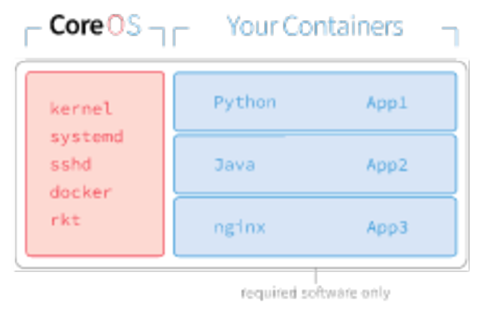
\includegraphics[width=\linewidth]{images/CoreOS}}
\caption{CoreOS container layout. \cite{www-core} \CE}
\label{fig:false-color}
\end{figure}

The company that \TODO{What company is that? You haven't mentioned
  before.} provides CoreOS Linux also provides open source tools like
etcd, rkt and flannel. CoreOS also has commercial products Kubernetes
and CoreOS stack. In CoreOS linux service discovery is achieved by
etcd, applications are run on Docker and process management is
achieved by fleet. \TODO{Scope: How do these other techs relate to
  CoreOS itself? Furthermore, if someone reading your paper doesn't
  already know what Docker, etcd, rkt, etc are, this paragraph makes
  little sense. You should give more context on why using these tools
  in CoreOS achieves for the user.}

Big data projects in science or business involve processing of large
amount of data.  These big data projects are hosted on bare metal
servers \TODO{What are bare metal servers?} or on clouds. Big data
projects in science and in business sector can benefit from container
frameworks that provide flexibility, ease of deployment, adding or
removing container clusters based on
demand. \cite{julian2016containers} Since CoreOS Linux is designed to
be used in container frameworks, it makes it one of the candidates to
be included into big data projects software stack that has container
cluster infrastructure. \TODO{Like before, you need to provide a
  little context. If someone doesn't know what container frameworks
  are or why they're useful, this paragraph is not very useful. In
  addition, start the paragraph with that last sentence. Otherwise
  it's not initially clear why you're talking about big data.}

\section{CoreOS Architecture and Installation}

CoreOS linux is a minimal operating system where the OS and utilities
are one unit and applications are run on containers. \TODO{This
  sentence belongs in the introduction. We already know what CoreOS
  is, now you need to talk about more specific things.} CoreOS has 9
disk partitions. The disk partions are: 1) EFI-SYSTEM which contains
the bootloader and the partition type is VFAT. 2) BIOS-BOOT, ROOT-C
and the 7th partion these partions have no partion format and are
reserved for future use. 3) USR-A and USR- B are the active and
passive partions that container linux sits on. Only one of them can be
active at a time and partion type is EXT4 depending on which one is
active. 4) OEM has EXT4 as partition type and this is where OEM
platform related configurations like custom networking and running an
agent are stored. 5) OEM-CONFIG serves as an alternative place for an
OEM. 6) ROOT may have EXT4, BTRFS, or XFS as partion type and it is
used for keeping data which is persistent and this partion is
stateful. \cite{www-core} \CE

\TODO{Paragraph could use some more context: how is this structure
  different for other Linux flavors? What is the motivation for having
  this disk structure?}

CoreOS Linux comes bundled with etcd, Fleet and Docker. Service
discovery in CoreOS Linux is achieved by etcd. Key value store
\TODO{Again, need more context. What is a key value store and why is
  ther one in CoreOS?} on etcd is distributed and stored on all
machines that run CoreOS Linux. This service discovery capability
makes it easy to add or remove machines. There is a command line
interface that comes preinstalled on CoreOS linux called etcdctl that
can be used to change and get key value data from etcd using etcdctl
set and etcdctl get respectively. Another command that can be used for
setting and reading key value is curl.

Container management in CoreOS linux is made possible by Docker.
All applications run on Docker. Containers can be launched using
docker run command line interface. \GE

Fleet is the third component of CoreOS and it is used for management
of containers with Docker installed. Fleet is init system \TODO{What
  does that mean?}  and fleetctl command line interface can be used to
check the status of containers, start and stop
containers.\cite{www-coreOSquickstart}

Based on the information in this book \cite{coreOSBook} \CE, there is no package
manager for installing, upgrading, configuring softwares in CoreOS
. Softwares \TE are installed as containers in CoreOS operating
system. Inorder \SE to apply updates, CoreOS makes use of two root
partitions one is active and the other is passive.First the updates to
CoreOS are applied to passive partion and upon reboot all the updates
are applied to the active partition.

CoreOS can be installed on clouds from EC2, Rackspace, GCE or virtual
machines such as Vagrant, VMware, OpenStack or on physical servers
such as PXE, iPXE, ISO. \cite{www-coreOSquickstart} \CE Based on the
information provided on CoreOS site \cite{www-coreOSvagrant}, CoreOS
container can be setup using Vagrant. Vagrant, virtual machine
manager, can be used to run CoreOS on a single machine with Windows,
OS X or Linux operating systems. It is recommened to have Vagrant
version 1.6.3 or latest. Virtual machines by VirtualBox or VMware are
both supported by Vagrant.

\section{Licensing}

CoreOS Container Linux is an open source operating system . It is
comprised of other programs and documents developed by other
individuals and companies. All original components that are part of
CoreOS Container Linux are licensed under Apache 2.0.  The latest
version of CoreOS Container Linux is 1325.1.0. \cite{www-core} \CE

\TODO{In a paper like this, it doesn't make sense to say "the latest
  version," since you don't know when someone will read it. Better
  say, "at the time of writing, ..."}

\section{Performance}

In a study done by Purdue University \cite{julian2016containers},
performance tests between CoreOS 899.5.0 on Docker and Red Hat
Enterprise Linux 6.5 were performed. In their study, the tests were
run on 24-core AMD Opteron systems, with 2.1 GHz processors, 48 GB
memory and 10Gbps Ethernet connection.  For HPL performance tests the
results were “The native RHEL 6.5 system showed an average performance
of 7.839 GFLOPS, versus 7.811 GFLOPS in a containerized environment
(approximately a 0.4\% slowdown). ” \TODO{You need to paraphrase this using your own words} The netwrok throughput iperf was
used and the results were: “final upload throughput was 8.43 Gbps
under Docker (versus 8.26 Gbps in RHEL 6.5), with a download
throughput of 9.37 Gbps (versus 9.38 Gbps in RHEL 6.5). ” \TODO{Please, paraphrase using your own words.} Network File
System throughput was done using iozone and results are shown in
Figure 2:

\TODO{Don't include a colon after "Figure 2" assuming the figure will
  be positioned right after the text. You should write the paper not
  assuming where certain figures are going to be located on the
  page. This is common practice, since figure formatting can be
  different based on the specific conference or journal where it's
  published, and your figures may be placed elsewhere to comply with
  the specific format.}

\begin{figure}[htbp]
\centering
\fbox{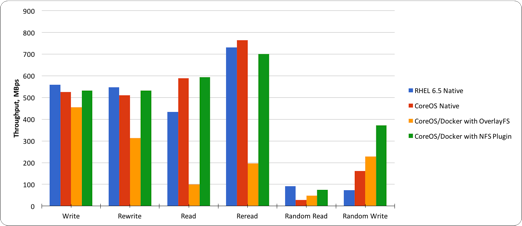
\includegraphics[width=\linewidth]{images/File-server-throughput}}
\caption{File Server throughput. \cite{julian2016containers} \CE}
\label{fig:false-color}
\end{figure}

In another study done in Institute of Informatics – Federal University
of Rio Grande do Sul \cite{2016NFVSolutions}, performance analysis of
ClickOS, CoreOS and OS\textsuperscript{v} was performed. “NFV is a new
networking paradigm where functions (e.g., firewalls, DNS, IDS),
traditionally performed by dedicated physical devices, are virtualized
and deployed on commodity hardware. ” \TODO{Please paraphrase} In
their paper comarision of ClickOS, CoreOS and OS\textsuperscript{v} as
NFV based tools was performed. They comapred \SE boot time, response
time and memory consumption for the three virtualization
technologies. As per their evaluation result, ClickOS has the lowest
boot time and response time followed by CoreOS and with regards to
memory cosumption, CoreOS has the smallest memory usage followed by
ClickOS. Based on the result OS\textsuperscript{v} has the slowest
boot time and response time as compared to CoreOS and ClickOS. Also
for memory consumption, OS\textsuperscript{v} has the highest
cosumption as compared to the other two technologies used.

\section{Use Cases}

In this section use cases from big data and other areas where CoreOS
Linux is used are discused \SE.

\subsection{Use Cases  for Big Data}

According to \cite{meyer2008metagenomics} \CE, Metagenomics RAST
server(MG-RAST) is free access portal that can be used by researchers
for accessing and analyzing metagenomics data. “Random community
genomes (metagenomes) are now commonly used to study microbes in
different environments. ” \TODO{Not relevant for this paper, and
  should be paraphrased if it was.} As described on
\cite{wilke2016mg}, CoreOS and fleet \TE are used on MG-RAST container
application servers. Researchers can input data into MG-RAST portal
through script, web site or REST API.

\subsection{Other Use Cases}
According to the paper \cite{2SPRA} \CE, CoreOS container linux \TE on
Amazon EC2 cloud was used to implement the project Two-stage
Stochastic Programming Resource Allocator (2SPRA). The language used
to implement was Python. In this project,they try \TODO{Avoid
  switching the tense between sentences.} to address the problem that
exist in most datacenters \SE of over provisioning resources in order to
achieve performance service level objective. 2SPRA is a resource
allocation scheme and it is able to optimize resource allocation for
containerized web services based on varying workloads. 2SPRA analyses
the relationship between change in workload, resource allocation and
response latency inorder to calculate the the number of containers
needed. In this experimental work, CoreOS was used inorder \SE to simulate
real word scenarios of n tier application servers running on
containers. The test architecture has client Java based emulator which
creates multiple user sessions at the same time, web hosting platform
with where RUBis benchmark is installed on Virtual machine with CoreOS
version stable r717.3.0 and the third component is 2SPRA implemented
in Python running on Virtual machine.


\section{Educational material} 

CoreOS website \cite{www-coreOSquickstart} \GE has detailed documentation
and materials for anyone who is interested in setting up CoreOS
Container linux on clouds, virtual or physical servers.  Users who are
interested can contribute to the CoreOS open source projects through
github \cite {www-coregit}.

This book \cite{coreOSBook} also has information about CoreOS overview
and its installation.

\section{Conclusion} 
CoreOS Linux is a light weight Linux based operating system that is
designed for containers. It provides abstraction by separating the
operating system from application and softwares. Operating system
updates to CoreOS are automatic without a need for user
interaction. CoreOS can be installed on clouds from EC2, Rackspace,
GCE or virtual machines such as Vagrant, VMware, OpenStack or on
physical servers such as PXE, iPXE, ISO.  

CoreOS Linux makes applications and microservices running on
containers secure, easy to deploy \TODO{"easy to deploy" is
  subjective; you can say that it \emph{aims to provide} easy to deploy
  applications and microservices, but the paper doesn't support that,
  so it ends up sounding like an advertisement} and portable. Big data
projects can leverage these benefits that comes with CoreOS Linux by
adding it to their infrastructure.

As previous performance results has shown \cite{2016NFVSolutions},
CoreOS Linux has the lowest memory usage compared to other
operating systems namely ClickOS and OS\textsuperscript{v}.


\section*{Acknowledgements}
The author would like to thank Professor Gregor von Laszewski and
associate instructors for their help and guidance.

% Bibliography

\bibliography{references}
 

\newpage

\appendix



\end{document}
